\section{Design}
\label{sec:design}
% This will give a description of the design.

% The organisation of this section should be the same as for the design documentation, and full details of the design are required. Typically it will comprise
    % a description of the anticipated components of the system and how they are to be organised;
    % a description of data structures used by the system;
    % algorithms to manipulate these data structures;
    % a design of the intended interfaces.
% Depending on the project and approach used, the followings are expected (refer to the guideline of the design stage for details):
    % Object-oriented design methodology:
    % Use-case diagrams; An interaction chart; The objects to be used in the system; Attributes and methods of objects; Pseudo-code for the key methods; Interface design.
    % Traditional design methodology:
    % Data dictionaries; System boundary diagrams; Entity-relationship diagrams; Logical table structures; Physical table structures; Transaction matrix; Pseudo-code for the key methods; Interface design.
    % Empirical investigation of hypothesis: in addition, the following is expected
    % A statement of the hypotheses to be tested; A description of the test data to be used; An experiment design, the experiments to be performed, any control to be used; A description of how the results will be analysed, including any statistical techniques that will be used; Anticipated conclusions.
    % Devising new algorithms: in addition, the following is expected
    % A description of the approach used to solve the problem; A description of how the new algorithms will be analysed, including mathematical and experimental analysis.
% All design documentation, representing the final design used on the project should be supplied.
% Any modifications made to the design presented in the design documentation and presentation should be stated and justified. ***

% It is often best to include the full details of the design as an appendix. In such a case, the design chapter in the main part of the project report should only discuss the most important elements of the design to your design report and state clearly what other elements will be given in the appendix.

% Keep in mind that examiners might not look at all the details of the material included in the appendices. So, make sure that the really important points of the design are explained here.

\subsection{Architecture}
Main idea is to generate variable datasets

\begin{figure}[H]
\centering
\caption{Main architecture}
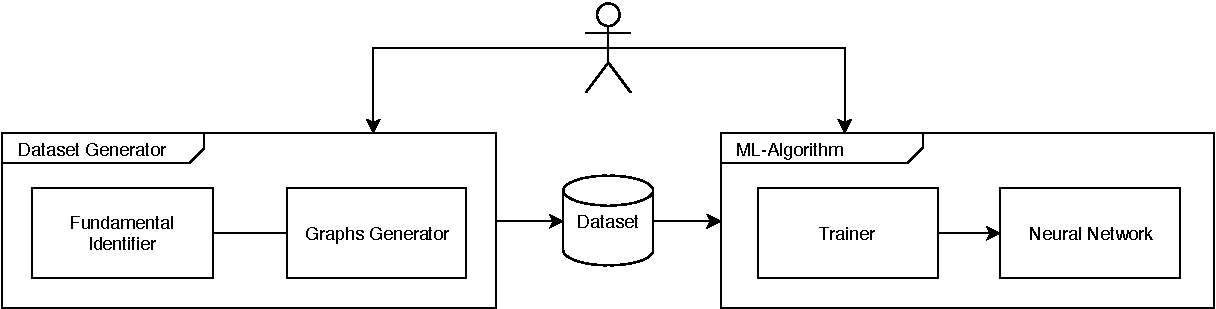
\includegraphics[width=\textwidth]{img/architecture.pdf}
\label{fig:global_performance}
\end{figure}



\subsection{Algorithm Design}
In this project, there are two algorithms involve. 
Both of them is used to check the existence of bisimulation relation between two given graphs.
The first one is a non-machine learning algorithm based on the work of Paige and Tarjan \cite{Paige1987}. 
The second algorithm is a neural network, training on the data that generated by the first algorithm.
\subsubsection{Traditional Bisimulation Algorithm}
Paige and Tarjan give the general solution of relational coarsest partition problem \cite{Paige1987}, which is identical to computing bisimulation equivalence \cite{Dovier2004}.
